\chapter{Conclusion}
\label{chap:conclusion}

\section{Selected Individual Firm Actions}
All the modeling techniques we tested are primarily targeted at identifying key relationships between firm-level actions and future decarbonization rates. Through our analysis, we had the opportunity to explore various important predictors, finding both expected and surprising results. In this section I will highlight the most important relationships, this will set the stage to then argue why these features can be useful to develop a better grading system for CDP reports. The results are presented in Table \ref{tab:results} where we show the coefficients of the Mixed Effect final model, as well as whether the variable was selected as important by the Bayesian Ridge and CatBoost models. We will primarily focus on variables that were selected as top 10 in importance by all three models. For a comprehensive overview of all the relationships, please refer to Chapter \ref{chap:chapter4}.


\subsection{Background Predictors}
Our analysis identified several core predictors essential for forecasting next-year's decarbonization rates. First among them is the \textbf{current-year decarbonization rates}, indicating a strong positive correlation with next-year's outcomes. This trend underscores a continuity in firms' environmental efforts, where entities engaged in emission reduction are likely to persist in their endeavors. Equally central to our analysis is the \textbf{industry} in which a firm operates. Our findings reveal that firms within sectors considered difficult to abate, such as \textbf{transportation} or \textbf{materials}, typically exhibit poorer decarbonization performance. Conversely, those in the \textbf{technology} and \textbf{consumer goods} sectors are more prone to reducing emissions, highlighting the impact of industry characteristics on decarbonization efforts and the need for tailored strategies across sectors.

Another significant predictor is the \textbf{geographical location}—both the \textbf{country} and \textbf{continent}—of a firm's operations. Our analysis points to a faster decarbonization pace within the \textbf{European Union}, as opposed to slower rates observed in \textbf{Asia}. This geographic variance is important to take into consideration when forecasting firm-level decarbonization rates, alongside an observed disparity in disclosure practices, with significantly more firms reporting in the \textbf{United States} and \textbf{Europe}.

Overall, the initial set of important variables for evaluating a company's future decarbonization trajectory include its \textbf{sector}, \textbf{country of operation}, and \textbf{current decarbonization rate}. Understanding these factors is an important starting point for assessing environmental strategies within the broader context of industry and geographic dynamics.

\subsection{Most Important CDP Survey Metrics}

In our analysis of CDP-specific metrics, certain predictors emerged as consistently significant across all models. These include the \textbf{average amount of emission targets} for Scope 1 and 2 emissions, the \textbf{verification method} for Scope 1 emissions, and the adoption of either a marginal abatement cost curve (MACC) or internal incentives to prioritize \textbf{emission reduction initiatives}.

Particularly important is the role of \textbf{incentive type} in predicting next-year's decarbonization rates, which according to our analysis is more significant than its impact on same-year rates. According to Table \ref{tab:results}, both \textbf{internal incentives} and the \textbf{MACC} approach show a negative correlation with decarbonization rates. This implies that firms employing these strategies tend to achieve greater year-on-year reductions in emissions. We find that having a good prioritization method to establish decarbonization initiatives is important, and has a greater impact on future decarbonization compared to impact on same-year decarbonization. This makes sense, as initiatives require a forward-looking approach with adequate time to plan, invest, and execute. Therefore, it is likewise important to have a proactive approach when evaluating initiatives, shifting from evaluating short-term impacts, which might not be significant, to assessing long-term outcomes. Therefore, based on our analysis, \textbf{we recommend that all key stakeholders interested in assessing future decarbonization rates should analyze which incentive structures are in place to determine the future effectiveness of a firm's environmental strategy, evaluating in particular whether or not a firm uses a Marginal Abatement Cost Curve or internal incentives to prioritize initiatives}.

\textbf{Scope 1 emission verification} also stands out as a crucial predictor. Firms that undertake comprehensive verification of their Scope 1 emissions are generally more successful in future decarbonization. This contrasts with outcomes associated with limited, moderate, unavailable, or third-party verification underway. This pattern underlines the value of external validation in emission reporting, suggesting that transparency and accountability in reporting, alongside consistent verification processes, are key to superior decarbonization performance. Firms that are open and accountable about their emissions tend to be more committed to environmental goals, reflecting a more structured and reliable strategy that is more likely to lead to decarbonization in the future. Therefore, \textbf{we find that the extent and rigor of emissions disclosure and verification serve as strong indicators of a firm's decarbonization commitment and effectiveness.}

Lastly, the \textbf{average amount of emission targets} set across Scope 1 and 2 emissions is an essential indicator of future decarbonization performance. \textbf{We find that firms that establish more ambitious targets are likely to demonstrate better decarbonization outcomes.} This consistency underscores the notion that ambition in setting environmental targets correlates with a firm's dedication to its environmental objectives and its capability to execute a sustained and effective strategy. Overall, based on our analysis, the level of ambition in emission targets is a direct indicator of a firm's potential to achieve significant decarbonization in the future.

\begin{table}[H]
    \centering
    \caption{Mixed Effects Coefficients and Feature Importance Indicators}
    \label{tab:results}
    \begin{tabular}{|l|c|c|c|}
    \hline
    \textbf{Predictor} & \textbf{MixedEffect} & \textbf{BayesianR} & \textbf{CatBoost} \\
    \hline
    Year & \textcolor{green}{$-0.048$} & \xmark & \cmark \\
    \hline
    \textbf{Ghg.Change.Real} & \textcolor{red}{$0.186^{***}$} & \cmark & \cmark \\
    \hline
    Market.Cap & \textcolor{green}{$-0.398^{***}$} & \xmark & \xmark \\
    \hline
    Revenue & \textcolor{red}{$0.257^{***}$} & \xmark & \xmark \\
    \hline
    \textbf{Type.S1.Limited/Moderate} & \textcolor{red}{$0.358$} & \cmark & \cmark \\
    \hline
    \textbf{Type.S1.N.A} & \textcolor{red}{$0.720^{***}$} & \cmark & \cmark \\
    \hline
    \textbf{Type.S1.Third.Party.Underway} & \textcolor{red}{$0.713^{**}$} & \cmark & \cmark \\
    \hline
    Ghg.Verification.Scope3.Yes & \textcolor{green}{$-0.272$} & \xmark & \xmark \\
    \hline
    Ghg1 & \textcolor{red}{$0.125^{***}$} & \xmark & \cmark \\
    \hline
    Ghg2Location & \textcolor{green}{$-0.046^{*}$} & \xmark & \xmark \\
    \hline
    Ghg1.Na & \textcolor{red}{$1.614^{***}$} & \xmark & \cmark \\
    \hline
    Ghg2Market.Na & \textcolor{red}{$0.917^{***}$} & \xmark & \cmark \\
    \hline
    Methane.Emissions & \textcolor{red}{$0.082^{***}$} & \xmark & \xmark \\
    \hline
    \textbf{Method.IndInternal Incentives} & \textcolor{green}{$-1.722^{***}$} & \cmark & \cmark \\
    \hline
    \textbf{Method.IndMacc} & \textcolor{green}{$-0.712^{**}$} & \cmark & \cmark \\
    \hline
    \textbf{Cdp.Targetamount.Mean} & \textcolor{green}{$-0.334^{***}$} & \cmark & \cmark \\
    \hline
    Cdp.Targettype.Absolute & \textcolor{green}{$-0.158^{***}$} & \cmark & \xmark \\
    \hline
    Cdp.Aggregated.Risk & \textcolor{red}{$0.625^{***}$} & \xmark & \xmark \\
    \hline
    Cdp.Aggregated.Opp & \textcolor{green}{$-1.085^{***}$} & \cmark & \xmark \\
    \hline
    Absent.Cdp.Initiative & \textcolor{red}{$0.685^{**}$} & \xmark & \xmark \\
    \hline
    Investment.Counter & \textcolor{green}{$-0.254^{***}$} & \xmark & \xmark \\
    \hline
    \end{tabular}
    % make the notes smaller and justify them]
    \vspace{+0.3cm}
    \caption*{
        \textit{Notes: For the Mixed Effects Model, results are reported from model (30) in Chapter 5 \ref{tab:R10}, where green indicates a positive impact and red indicates a negative impact on decarbonization. Significance levels are denoted as *, **, and *** for p<0.1, p<0.05, and p<0.01, respectively. For the Bayesian Ridge and CatBoost models, the displayed feature importances are from the tuned models. A green check (\cmark) signifies that the feature is among the top 10 based on feature importance, whereas a red cross (\xmark) indicates it is not. Reference category for Type.S1 is Type.S1.Adequate, reference category for Method is Method.Other.}
    }
\end{table}

\section{Final Modeling and Data Considerations}

We found that, based on our data detailed in Chapter \ref{ch:data-sources}, building a universal model that accurately forecasts decarbonization rates for any specific firm through disclosure and financial data is not achievable. Due to irregularities in disclosure, such as missing values, non-accurate figures, and inherent variability not captured by disclosure data, there is not enough forecasting power to accurately predict next year decarbonization for a specific firm. To illustrate this point, it is sufficient to observe the various figures presented in Chapter \ref{chap:chapter4} where it is possible to observe significant noise in our data.

Though, we are successful in achieving our to major objectives. As explained in the introduction, the focus of predictive modeling is twofold: first, we want to understand which models work best with disclosure data when it comes to forecasting decarbonization rates at the firm-level. Second, through a predictive exercise, our aim is to identify which predictors are significant across various modeling techniques and what is their correlation with future decarbonization. 

Addressing the first question, we found that more interpretable modeling techniques, such as Mixed Effects and Bayesian Regression, are the best choice. Alternatively, models that are particularly capable at leveraging categorical data are also valid choices, with tree-based model and CatBoost yielding the best results. \textbf{We found that any model that (i) either requires a relatively large number of data-points per firm to train (Long-Short Term Memory, Autoregressive Integrated Moving Average) or (ii) that does not perform regularization and is not able to handle categorical data with high number of categories (Ordinary Least Squares) should be avoided}. The first group's disadvantage is obvious: we do not gain better predictive results compared to Mixed Effects as on average each firm does not have more than six data-points, and we have less interpretability. Arguing why we should not use simple linear models which are standard in the field is more nuanced: first, we through our analysis we found that it is important to place each firm in its own category and recognize the profound difference in operations between firms that operate in different industries, countries, and continents. Yet, this in a traditional setting would require a significant number of columns and if we one-hot-encode all this information we risk over-fitting to the data. Second, if we instead chose not to use all those categorical information to prevent over-fitting, then we bias some of the important relationships we are trying to uncover as we do not control for the fact that each firm has its own unique characteristics, and we build models that are not representative of the structure of our data thus we encounter an important omitted variables problem. 


The most important key takeaway of predictive modeling is that \textbf{when it comes to disclosure data, taking a forward-looking predictive approach allows to uncover firm-level disclosure actions that correlate with future decarbonization, which we would miss in a traditional same-year inference setting}.  Crucially we need individual firms to decarbonize, thus it is important to suggest to all stakeholders which actions are most likely to lead to decarbonization \textbf{at the firm level}. Therefore,
\textbf{we should not aggregate the data}, as although we would likely get a better prediction of the aggregated emissions as is typically the case when aggregating, this will not actually be useful in practice for suggesting individual firm actions as aggregating can lead to the data showing a different relationship  due to Simpson's paradox \cite{pearl2013understanding}. That is, we risk observing a trend or result that is present when data is put into groups that reverses when the data is combined \cite{simpsons, pearl2013understanding}. If we rather are interested in a specific sector, then the best approach would be to build a sector specific model, still leveraging data at the firm-level.

\begin{figure}[H]
    \centering
    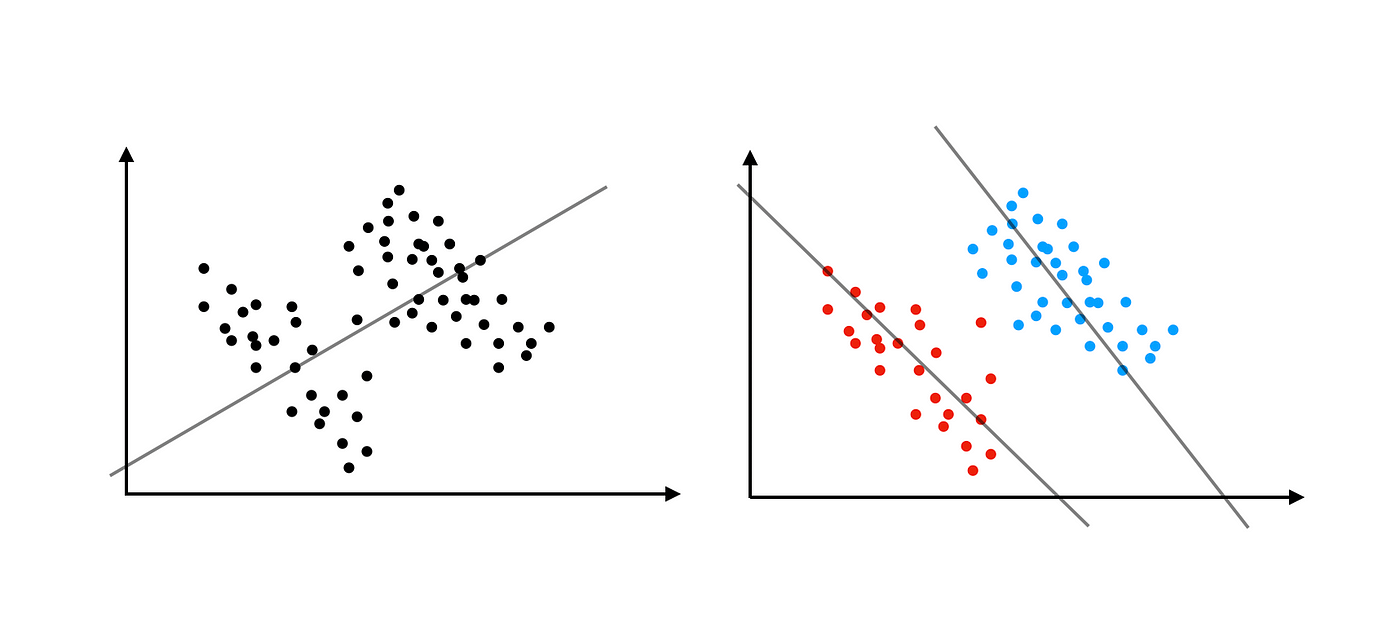
\includegraphics[width=0.7\textwidth]{thesis_tex/figures/simpson.png}
    \caption{Illustration of Simpson's Paradox. Adapted from \cite{simpsons}}
    \label{fig:simpson}
\end{figure}

Addressing the second question, we present our main models, Mixed Effects, Bayesian Ridge, and CatBoost regression outlined in Chapter \ref{ch:finding-the-best-model} to serve as benchmark for modeling CDP data specifically to assess firm-level strategies and identifying key predictors. We believe that these models are important not only for their predictive ability, but for guiding future research and understanding how to answer crucial questions on what matters the most when it comes to decarbonizing. 



% This task would be better achieved  our goal was to determine the decarbonization rate of a specific firm with great precision then we would likely need more predictors with higher frequency than yearly disclosure and financial data, and a firm-specific model (or the work of a specialized analyst) would probably to outperform any general model. 



% Instead, we focused on understanding which specific firms \textbf{individual firm actions} correlate with future decarbonization.







% This is because disclosure data at the firm level is effectively a multiple timeseries problem, where each firm represent one timeseries and our interest is to understand what the effect of predictors is across firms. Notably, each timeseries only has on average six data points (of the firms in our dataset, each has reported to the CDP for an average of 6 years as of 2022), therefore models such as LSTM (Long-Short Term Memory) Neural Networks, which are typically applied when forecasting timeseries, are not useful as there is not enough data-points to train. Furthermore, due to irregularities in reporting, such as missing values, non-accurate figures, and inherent variability not captured by disclosure data, there is not enough forecasting power to accurately predict next year decarbonization for a specific firm. 

% We found that the key is to leverage the panel aspect of our data, with firms belonging to sevaral industries, countries, contients, and with each firm reporting multiple years. Additionally, we found an incredible opportunity to identify important predictors across firms by using models that can take into consideration the fact that each firm has its own unique characteristics, while at the same time allowing for general trends to emerge. Crucially, the opportunity is in uncovering the underlying mechanisms that drive emissions reductions derived from \textbf{individual firm actions} and that are valid across a range of firms. This is extremely important as there is not enough 

% Thus we found that the best approach is to have models that prioritize explainability, and that also have the ability to model firm-specific behavior on one hand, and on the other hand to borrow strenghts across firms to determine trends.

% Thus, we found that two models are particularly useful: Mixed Effects and CatBoost regression. 


%  We found that the structure of disclosure data lends more effectively to uncovering key relationships and dynamics within the decarbonization process, rather than focusing solely on predicting exact future emissions for individual firms—a task made challenging without high-frequency data and better addressed with firm-specific models. We therefore focused on using a predictive framework for identifying the key predictors of next-year decarbonization, 
  
 
%  his approach allowed us to uncover the underlying mechanisms that drive emissions reductions derived from \textbf{individual firm actions} and that are valid across a range of firms. Overall, I believe that true value of disclosure data is not in predicting future emissions for any specific firm, but in understanding which actions correlate with future decarbonization which, if acted upon, can lead to significant emissions reductions at the firm level. In this regard, an important consideration to make is that, as explained in the introduction, we need individual firms to decarbonize, thus it is important to suggest to all stakeholders which actions are most likely to lead to decarbonization at the firm level. Therefore, we should not aggregate the data, as although we would likely get a better prediction of the aggregated emissions, this could lead to the aggregated data showing a different relationship than the individual data (Simpson's paradox) \cite{pearl2013understanding}.

% To build a good predictive model at the firm-level, we found to leveraging the panel data format to be the most important aspect. As we want to take into consideration the individual firm characteristics, without overly increasing the dimensionality of the data. Within this context, Mixed Effects models and CatBoost emerged as standout methodologies. Their superior handling of categorical data allowed us to tap into the full potential of repeated measurements over time, enabling an exhaustive exploration of how various strategies impact firm-level emissions.

% Crucially, the use of random intercepts in Mixed Effects models played an important role in our analysis. This approach allowed us to account for intrinsic firm characteristics when assessing the influence of different predictors on emissions by creating a random intercept for every firm. By isolating the effects of these variables, we could ensure that the observed relationships were not reflections of underlying firm attributes but rather genuine indicators of strategic impact across all firms. This new understanding of predictor effects, controlled for individual firm characteristics, highlights the incredible potential of using disclosure data to inform decarbonization strategies and policies for individual firms.


\section{Enhancing the CDP Survey}

\subsection{Addressing Missing Data}
Our research, particularly the insights gained from the residuals plots in Figures \ref{fig:mixed_effects_residuals} and \ref{fig:bayesian_ridge_residuals}, highlights a significant challenge: accurately reporting changes in emissions over time when data is missing. The noticeable diagonal trends in both plots reveal the models' difficulties in predicting zero-emissions changes. Upon examining the disclosure reports, it becomes evident that many companies inadequately respond to question (C7.9a), \textit{"Identify the reasons for any change in your gross global emissions (Scope 1 and 2 combined), and for each specify how your emissions compare to the previous year"}, often providing minimal information. Figure \ref{fig:missing_data} exemplifies this issue, showing reported emissions changes without the corresponding percentage changes. This omission hinders the ability to assess decarbonization efforts and adversely affects model predictions. Excluding such data is an alternative; however, it restrictively narrows our analysis to a minute fraction of companies that consistently report percentage changes across all categories.

Consequently, I recommend that the CDP survey should emphasize the importance of reporting percentage changes in its guidelines. \textbf{Rather than defaulting to a zero value, there should be an option to indicate a "change not measured" category}. This distinction would clarify the difference between actual zero percentage changes and unmeasured changes, which are currently indistinguishable. A practical solution could involve enhancing the survey with a drop-down menu accompanying the numerical entry field, where the default option is "change not measured" instead of a blank space. This modification would rectify the confusion and is straightforward to implement, ensuring a clearer differentiation between companies that accurately report zero changes and those that do not measure such changes.


\begin{figure}[H]
    \centering
    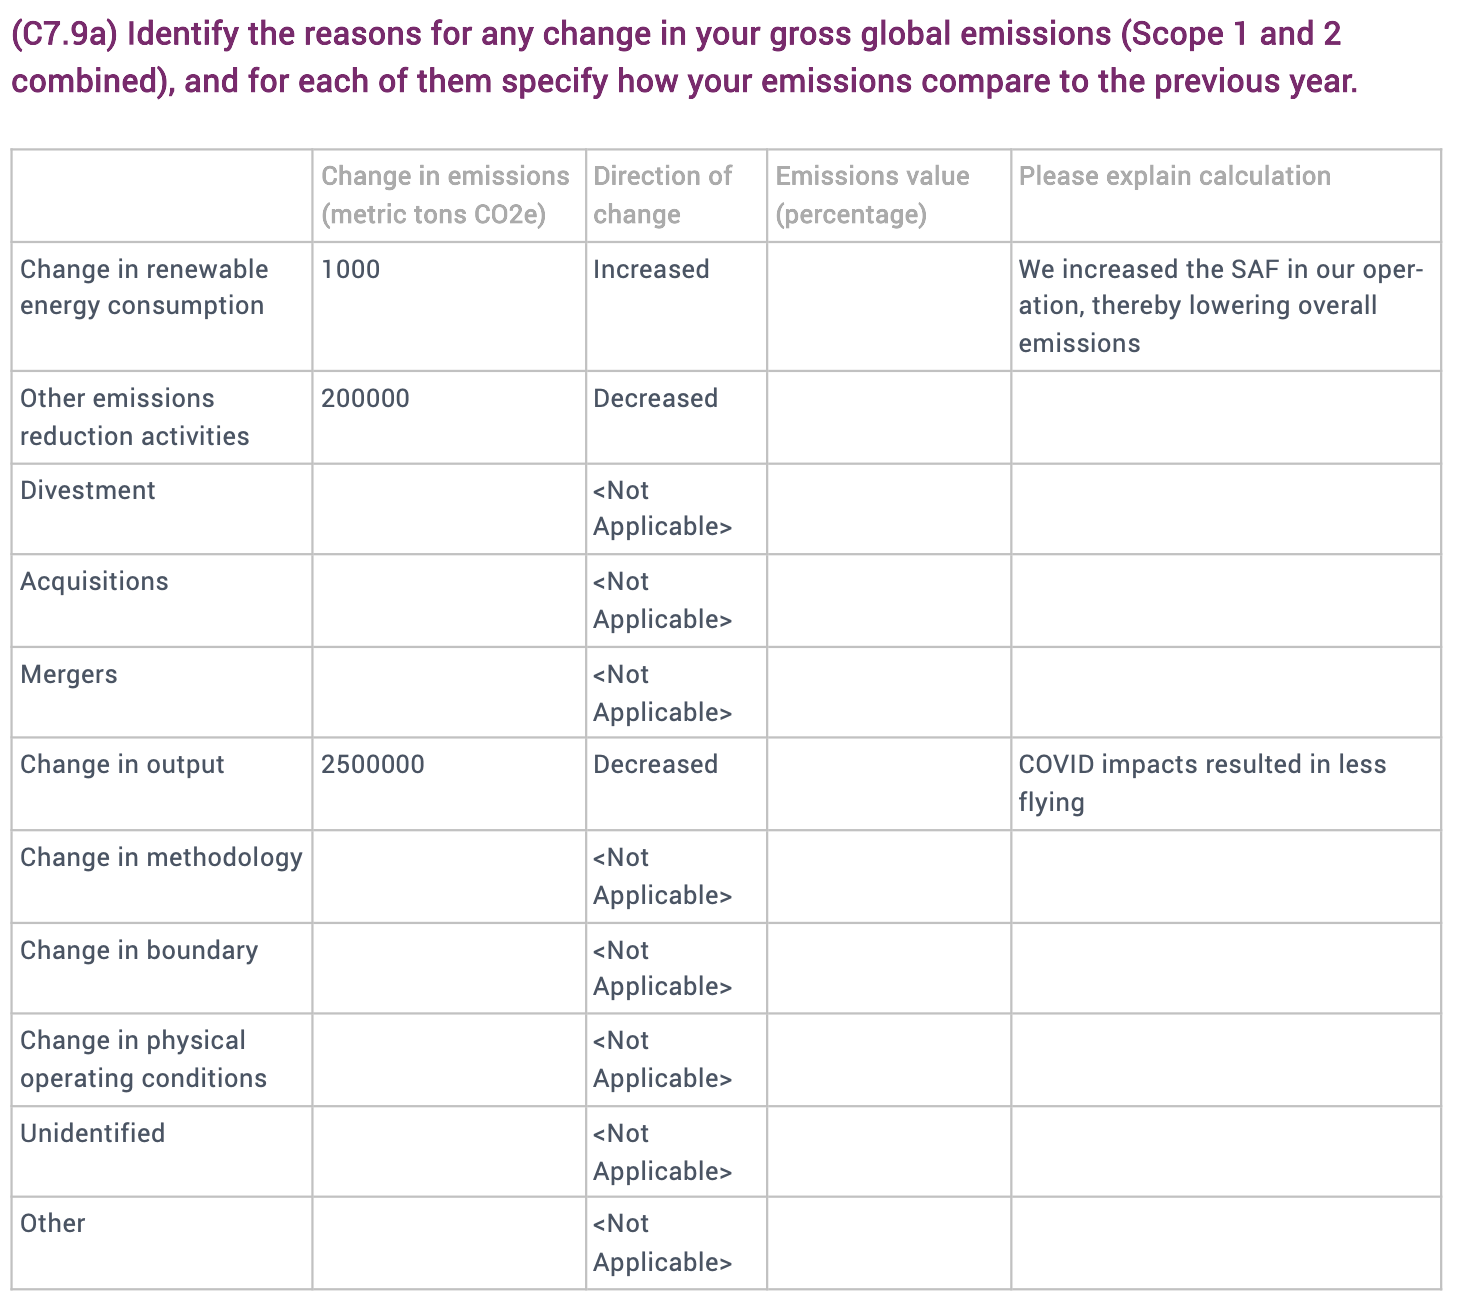
\includegraphics[width=0.7\textwidth]{thesis_tex/figures/cdp_missing.png}
    \caption{Example of Missing Data in Question C7.9a}
    \label{fig:missing_data}
\end{figure}





% In this section, based on our results, we will provide an actionable recommendation to enhance the design of the CDP climate survey to promote decarbonization. I am aware that there are multiple considerations, such as consistency, ease of complying, and adaptability across sectors, that influence the design of the survey, and I also recognize that statistical analysis is not the only priority. Therefore, rather than suggesting changes to the actual questions, I will propose a simple additions,  that would greatly aid in enhancing statistical models. A major problem encountered when modeling is missing data when it comes to reporting 


% Discussion on the residuals -> missing data is the problem -> we can use this as a feature to enhance disclosure. Simple surveys with pinpointed questions. 

\subsection{CDP Scores: a forward looking approach}
Concluding our analysis, I propose a \textbf{streamlined decision tree designed to evaluate a firm's decarbonization efforts, categorizing them as either a decarbonization leader, aware, or novice}. This categorization leverages the critical predictors identified earlier and acknowledges the prevalent issue of incomplete data in decarbonization rate assessments. A ``decarbonization leader'' is a firm our analysis predicts will achieve decarbonization, demonstrating significant commitment through action on key predictors and exhaustive reporting of decarbonization rates. The ``decarbonization aware'' category includes firms that acknowledge decarbonization by reporting decarbonization rates yet show minimal initiative towards future commitments. Lastly, the ``decarbonization novice'' category comprises firms that do not disclose decarbonization rates, indicating they are significantly behind and in need of revising their current strategies. \\~\\

\begin{figure}[H]
\centering
\begin{forest}
    for tree={
        draw,
        rounded corners,
        align=left,
        edge={->},
        parent anchor=south,
        child anchor=north,
        l sep+=1.2cm, % Increase the level distance
        scale= 0.8,
        edge label={node[midway, fill=white, font=\sffamily\small]},
    },
    [Does the firm report \% decarbonization rates?, fill=blue!20
        [Decarbonization Novice, fill=red!20, edge label={node[midway, left] {NO}}]
        [Does the firm have exhaustive\\Scope 1 verification?, fill=blue!20, edge label={node[midway, right] {YES}}
            [Decarbonization Aware, fill=yellow!20, edge label={node[midway, left] {NO}}]
            [Does the firm use a MACC and/or\\internal incentives?, fill=blue!20, edge label={node[midway, right] {YES}}
                [Decarbonization Aware, fill=yellow!20, edge label={node[midway, left] {NO}}]
                [Decarbonization Leader, fill=green!20, edge label={node[midway, right] {YES}}]
            ]
        ]
    ]
\end{forest}

\captionof{table}{Decision Tree to Assign Decarbonization Scores}
\label{fig:grading-tree}
\end{figure}




\section{Future Work}
I am incredibly grateful to conclude this thesis having at the same time a better understanding on what it takes to achieve impact in terms of decarbonization, and so many more ideas and questions on further areas to explore with respect to disclosure data, and leveraging statistical models to advance our understanding of firm-level emissions. I am confident that the study of emissions at the corporate level will be ever-more popular as we need businesses to decarbonize. 

\textbf{I hope that if there is one element that the kind reader will take away from this work is the enormous opportunity of using disclosure data to answer important questions about future emissions focusing at the firm-level.} As showed in this thesis, we already have enough data to answer important questions, and we can apply statistics and computer science methods to gain important insights and further increase transparency. Our challenge is a two-sided quest: on one hand we need firms to disclose their data, and on the other we need to be able to leverage the data to enhance disclosure itself, by asking increasingly more effective questions, and to provide businesses with clear guidance on how to successfully decarbonize. 

There are many avenues in which we can further advance our research: first and foremost, we can test how the impact of certain predictors changes as we shift our time horizon. As we found in our thesis, \textbf{internal incentives} is correlated to more decolonization on a next-year basis compared to a same-year basis. It would be very interesting to observe this relationship looking multiple years out. This same analysis can be applied to any predictor of interest, analyzing the significance and relationship with decarbonization over time. 

Another interesting avenue is to build \textbf{industry-specific models} that replicate this analysis at the firm-level only considering businesses that operate in a specific industry. Such a model could be able to pinpoint even more precise relationships that are true for a given industry, with the potential of providing more tailored recommendation. The advantage of this task is that the same models can be used, the only variable to change is the data, by filtering only one industry. 

Finally, it would also be interesting to see how the proposed scoring of decarbonization efforts based on our decision tree at Figure \ref{fig:grading-tree} compares to CDP grades, and whether our forecasting model predict firms with a better CDP to decarbonize more. It would be very interesting to look at similarities and differences between those two methods, prediction and scoring, to understand whether scoring could benefit from insights from a forward-looking approach, as I attempted to suggest in this work.